\documentclass[a4paper,12pt]{article}
\usepackage[slovene]{babel}
\usepackage[utf8]{inputenc}
\usepackage[T1]{fontenc}
\usepackage{lmodern}
\usepackage{amsmath,amsfonts,amssymb}
\usepackage[ruled,vlined]{algorithm2e}
\usepackage{graphicx}
\usepackage{subfigure}
\usepackage{matlab-prettifier}
\usepackage{enumitem}
\usepackage{hyperref}

\title{\textbf{\huge Aproksimacija spodnjega dela krožnice s Hermiteovo interpolacijo}
	
	\Large \it Poročilo o projektni nalogi pri predmetu Matematično modeliranje}
\author{Urša Kumelj}

\begin{document}
	
	\maketitle
	
	\tableofcontents

	\newpage

	\section{Naloga}
	Denimo, da potuje kroglica pod vplivom gravitacije (brez trenja) iz točke $\boldsymbol{T}_1 = \frac{1}{\| (-1,b) \|} (-1,b)$ v točko $\boldsymbol{T}_2 = \frac{1}{\|(1,-b)\|}(1,-b)$, $b \in \mathbb{R}$, $b>0$, po
	kubični B\'{e}zierjevi krivulji $\boldsymbol{p}$, ki aproksimira spodnji del krožnice, katera
	ima središče v izhodišču in gre skozi $\boldsymbol{T}_1$ ter $\boldsymbol{T}_2$. Določite iskani enostranski Hermiteov interpolant $\boldsymbol{p}$, tj. kubično B\'{e}zierovo krivuljo, ki zadošča Hermiteovim interpolacijskim pogojem in ima parameter 
	$L = \frac{4}{3} \tan(\frac{1}{4}\alpha)$ ter odgovorite na naslednja vprašanja.
	\begin{enumerate}[label=(\alph*)]
		\item Koliko je kroglica oddaljena od koordinatnega izhodišča pri parametru $t = \frac{1}{2}$?
		\item Katera je najnižja točka, ki jo doseže kroglica med potovanjem po $\boldsymbol{p}$?
		\item Kakšna je absolutna vrednost hitrosti kroglice, ki potuje po $\boldsymbol{p}$, ko
		pride v točko $\boldsymbol{T}_2$?

	\end{enumerate}

	
	\section{Matematično ozadje}
	
	\subsection{B\'{e}zierjeve krivulje}
	
	B\'{e}zierjeve krivulje so parametrične krivulje, pomembne v računalniški grafiki. Določene so z zaporedjem kontrolnih točk.
	Osredotočili se bomo le na kubične B\'{e}zierjeve krivulje. Te so sestavljene iz štirih kontrolnih točk $\boldsymbol{P}_0, \boldsymbol{P}_1, \boldsymbol{P}_2, \boldsymbol{P}_3$ in imajo obliko
	\begin{equation*}
		b(t) = \boldsymbol{P}_0(1-t)^3 + 3\boldsymbol{P}_1(1-t)^2t + 3\boldsymbol{P}_2(1-t)t^2 + \boldsymbol{P}_3t^3, \quad t \in [0,1]
	\end{equation*}
	Pomembne lastnonosti B\'{e}zierjevih krivulj so: 
	\begin{enumerate}[label=(\roman*)]
		\item Prva in zadnja kontrolna točka sta interpolacijski: 
		$$b(0) = \boldsymbol{P}_0,\quad b(1) = \boldsymbol{P}_3.$$
		\item Tangentna vektorja v prvi in zadnji točki sta
		$$b'(0) = 3(\boldsymbol{P}_1 - \boldsymbol{P}_0),\quad b' = 3(\boldsymbol{P}_3 - \boldsymbol{P}_2).$$
		\item Krivulja leži v konvekcijski ovojnici kontrolnih točk.

	\end{enumerate}
	
	\subsubsection{De Casteljaujev algoritem}
	
	Postopek vsaki vrednosti parametra $t \in [0,1]$ učinkovito priredi točko na B\'{e}zierjevi krivulji. Geometrijsko gledano je de Casteljajev algoritem ponavljanje linearnih interpolacij.
	Implementacija v Matlabu je naslednja:
	\begin{lstlisting}[style=Matlab-editor,numbers=left]
function tocka = deCasteljau(b,t)
  n = size(b,2);
  for i = 2:n
  b = (1-t).*b(:,1:end-1) + t.*b(:,2:end);   
  end
  tocka = b(:,end);
end
	\end{lstlisting}
	
	
	\subsubsection{Enostranski Hermiteov interpolant}
	
	Za aproksimacijo krožnih lokov z enostranskim Hermiteovim interpolantom tipično določimo točke na krožnici, ki jih želimo interpolirati, 
	in tangentne vektorje v teh točkah, ki so usmerjeni vzdolž tangent na krožnico v teh točkah. Ideja pri tej metodi je potisniti srednjo točko v $0$. 
	Vrednsot parametra $L$, ki ustreza enostranskemu Hermiteovemu interpolantu, je tako $L = \frac{4}{3} \tan(\frac{1}{4}\alpha), \alpha \in [0,2\pi]$.
	Kako dosežemo to vrednost? 
	
	\noindent\hspace*{10em}
	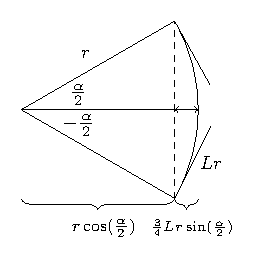
\includegraphics[scale=1.5]{slika.pdf} 
	
	
	Iz slike vidimo, da je razdalja od izhodišča do sredine loka enaka 
	$$r\cos(\frac{\alpha}{2}) + \frac{3}{4}Lr\sin(\frac{\alpha}{2}).$$
	Mi bi želeli dobiti tak parameter $L$, da bo zgornja razdalja enaka radiju $r$.
	\begin{eqnarray*}
		r &=& r\cos(\frac{\alpha}{2}) + \frac{3}{4}Lr\sin(\frac{\alpha}{2})\\
		L &=& \frac{3}{4} \cdot \frac{1-\cos(\frac{\alpha}{2})}{\sin(\frac{\alpha}{2})} = \frac{3}{4}\tan(\frac{\alpha}{4})
	\end{eqnarray*}
	
	\section{Reševanje}
	\subsection{Implementacija naloge}
	
	Začnimo z implementacijo same naloge in nato rešimo preostale podnaloge.
	Potrebujemo aproksimacijo spodnjega dela krožnice iz točke $\boldsymbol{T}_1$ do $\boldsymbol{T}_2$, ki sta normirani, kar pomeni, da ležita na enotski krožnici.
	Problem bomo rešili tako, da bomo aproksimirali lok krožnice iz točke, ki leži v četrtem kvadrantu do točke, ki leži v prvem kvadrantu. 
	Dobljeno implementacijo bomo potem zarotirali za določen kot, da bomo dobili ravno željeno. Vmesni kot med točkama pa je vedno $\pi$.
	\\
	Najprej potrebujemo določiti kontrolne točke kubične B\'{e}zierove krivulje. Torej za prvo kontrolno točko vzemimo $\boldsymbol{P}_0 = (-\cos(\varphi), -\sin(\varphi))$, 
	ki je točka v četrtem kvadrantu na krožnici in 
	$\boldsymbol{P}_3 = (\cos(\varphi), \sin(\varphi))$ kot zadnjo kontrolno točko, ki je v prvem kvadrantu. Kot $\varphi$ je polovični kot med njima, zaradi simetrije.
	Da bo ta krivulja zadoščala enostranskemu Hermiteovemu pogoju, mora biti odvod usmerjena tangenta same krožnice.
	Tako bosta preostali dve kontrolni točki oblike $\boldsymbol{P}_1 = \boldsymbol{P}_0 + L\boldsymbol{P}'_0$ in $\boldsymbol{P}_2 = \boldsymbol{P}_3 - L\boldsymbol{P}'_3$, kjer je $\boldsymbol{P}'_0 = (\sin(\varphi), -\cos(\varphi))$, $\boldsymbol{P}'_3 = (-\sin(\varphi), \cos(\varphi))$ in
	$L = \frac{4}{3} \tan(\frac{1}{4}\pi)$, ki določa dolžino tangentnega vektorja v krajiščih.
	\\
	Da dobimo spodnji del krožnice, je potrebna rotacija za kot $-\frac{\pi}{2}$, za pravilno postavitev 
	točk $\boldsymbol{T}_1$ in $\boldsymbol{T}_2$ pa lahko kot dobimo na naslednji način. Ker poznamo koordinati točke, lahko preprosto s trigonometrijo dobimo
	$$\tan(\phi) = \frac{y}{x} = \frac{b}{-1} \Leftrightarrow \phi = \arctan(-b).$$
	Implementacija v Matlabu:
	
	\begin{lstlisting}[style=Matlab-editor,	numbers=left,]
function c = aproksimacija_kroznice(b)
 fi = pi/2;
		
 T1 = [-cos(fi); -sin(fi)];
 T2 = [cos(fi); sin(fi)];
 dT1 = [sin(fi); -cos(fi)];
 dT2 = [-sin(fi); cos(fi)];
		
 L = 4/3*tan(pi/4);
		
 c = [T1,T1+L*dT1,T2-L*dT2,T2];
		
 kot_rotacije = atan(-b)-pi/2;
 M = [cos(kot_rotacije),-sin(kot_rotacije);sin(kot_rotacije),cos(kot_rotacije)];
 c = M*c;
 plotBezier(c); 
 axis equal;
end
	\end{lstlisting}
	
	\noindent V implentaciji je uporabljena funkcija \lstinline[style=Matlab-editor]!plotBezier!, ki nam krivuljo izriše.
	
	\begin{figure}[h]
		\centering
		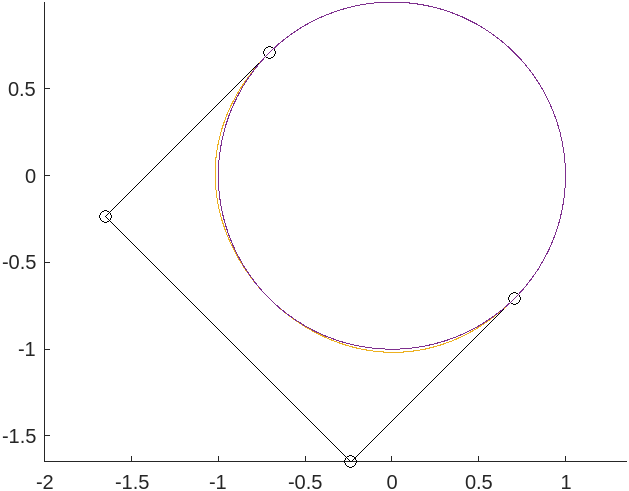
\includegraphics[scale=0.7]{slika2.png}
		\caption{Primer aproksimacije spodnjega dela krožnice pri $b = 1$ ter hkrati izris enotske krožnice.}
	\end{figure}
	
	
	\subsection{Rešitev točke a)}

	Glede na to, kako je izračunan parameter $L$, bo razdalja pri $t=\frac{1}{2}$ vedno enaka radiju krožnice, torej $1$, saj smo na enotski
	krožnici. Rezultat pa lahko seveda preverimo v Matlabu. S pomočjo funkcije \lstinline[style=Matlab-editor]!deCasteljau! izračunamo točke na krivulji pri
	parametru $t$.

	\begin{lstlisting}[style=Matlab-editor,	numbers=left,]
 b = 1;
 t = 1/2;
 kontrolne_tocke = aproksimacija_kroznice(b);
 tocka = deCasteljau(kontrolne_tocke,t);
 razdalja = sqrt(tocka(1)^2 + tocka(2)^2)
	\end{lstlisting}

	\noindent Seveda parameter $b$ poljubno spreminjamo. 

	\subsection{Rešitev točke b)}
	Najnižja točka, ki jo doseže kroglica med potovanjem po $\boldsymbol{p}$ izračunamo s pomočjo vgrajene funkcije \lstinline[style=Matlab-editor]!fminsearch!. Glede na to, da točke na 
	B\'ezierjevi krivulji pridobivamo z De Casteljaujevim algoritmom, kjer parameter $t$ točno določa posamezno točko, je potrebno poiskati, pri katerem $t$ je dosežen minimum. Za iskanje minimuma pa so
	pomembne le ordinate kontrolnih točk, zato sem uporabila funkcijo \lstinline[style=Matlab-editor]!deCast!, ki deluje le na vektorju kontrolnih točk $b$ velikosti $(n+1)$. Na koncu je potrebno dobljeni $t$ vstaviti v  
	De Casteljajev algoritem, da dobimo konkretno točko minimuma in jo na sliko tudi narišemo z ukazom \lstinline[style=Matlab-editor]!scatter!.

	\begin{lstlisting}[style=Matlab-editor,	numbers=left,]
function tocke = deCast(b,t)
 [~,n] = size(t);
 [~,m] = size(b);
 tocke = zeros(1,n);
 b_nov = b;
 for i=1:n
   b_nov = b;
   for j=1:m-1
    [~,l] = size(b_nov);
    b_nov = b_nov(1:l-1).*(1-t(i)) + b_nov(2:l).*t(i);
   end
 tocke(i) = b_nov;
end
\end{lstlisting}


	\begin{lstlisting}[style=Matlab-editor,	numbers=left,]
 kontrolne_tocke_y = kontrolne_tocke(2,:);
 funkcija = @(t) deCast(kontrolne_tocke_y,t);
 iskani_t = fminsearch(funkcija,0.7);
 minimum = deCasteljau(kontrolne_tocke, iskani_t)
 scatter(minimum(1), minimum(2), 10, 'filled', 'MarkerEdgeColor', 'k', 'MarkerFaceColor', 'g')
	\end{lstlisting}

	\clearpage

	\begin{figure}[h!]
		\centering
		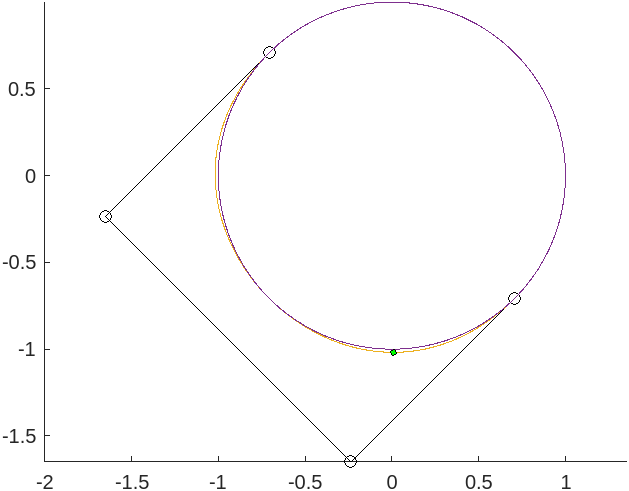
\includegraphics[scale=0.7]{slika3.png}
		\caption{Izris minimuma na aproksimacijo spodnjega dela krožnice pri $b = 1$ ter hkrati izris enotske krožnice.}
	\end{figure}
	
	\subsection{Rešitev točke c)}
	
	Za izračun hitrosti velja enačba $v = \sqrt{2g(-y)}$, ki velja zaradi zakona o ohranitvi energije. 
	Kot pri prejšnji točki tudi tukaj že iz enačbe vidimo, da potrebujemo zgolj $y$ komponente točk na krivulji, zato bomo
	uporabili funkcijo \lstinline[style=Matlab-editor]!deCast!. Vse $y$ kontrolne točke sedaj enostavno vstavimo v enačbo za hitrost in
	jo izračunamo za vsak $t \in [0,1]$. Na koncu vrnemo le absolutno vrednost zadnjega elementa vektorja, saj je pri $t = 1$ dosežena točka $\boldsymbol{T}_2$.

	\begin{lstlisting}[style=Matlab-editor,	numbers=left,]
 g = 9.81;
 t = linspace(0,1);
 y_tocke_krivulje = deCast(kontrolne_tocke,t);
 v = abs(sqrt(2*g*(-y_tocke_krivulje(end))))
	\end{lstlisting}
	

	\section{Viri in literatura}
	
	\begin{enumerate}[label=\textbullet]
		\item Zapiski s predvanj in vaj pri predmetu Matematično modeliranje, vse je dostopno na letošnji spletni učilnici kot tudi na učilnicah preteklih let.
		\item Wikipedia o B\'{e}zierjevih krivuljah, dostopno na \href{https://sl.wikipedia.org/wiki/Bézierova_krivulja}{Wikipedia}.
		\item Calculate control points of cubic bezier curve approximating a part of a circle, dostopno na \href{https://math.stackexchange.com/questions/873224/calculate-control-points-of-cubic-bezier-curve-approximating-a-part-of-a-circle}{StackExchange}.
		\item Git repozitorij Nika Erzetica, dostopno na \href{https://github.com/nikerzetic/matematicno-modeliranje}{GitHub}.
	\end{enumerate}
	
\end{document}